% docx2tex 1.5 --- ``Keep your distance and avoid spreading Word'' 
% 
% docx2tex is Open Source and  
% you can download it on GitHub: 
% https://github.com/transpect/docx2tex 
%  
\documentclass[a4paper,12pt]{article}
\usepackage[table]{xcolor}
\usepackage[T1]{fontenc} 
\usepackage[utf8]{inputenc} 
\usepackage{wrapfig}
\usepackage{graphicx} 
\usepackage[hidelinks]{hyperref}
\usepackage{multirow} 
\usepackage{color} 
\usepackage{textcomp} 
\usepackage{amsmath}  
\usepackage{enumerate} 
\usepackage{tensor} 
\usepackage[slovene,english]{babel}
\usepackage{tikz}
\usetikzlibrary{positioning,calc}
\usepackage{geometry}
\geometry{left=25mm,top=28mm,right=25mm,bottom=28mm}
\usepackage{titletoc}
\usepackage{ragged2e}
\usepackage[labelfont=bf]{caption}
\usepackage{lastpage}
\usepackage{fancyhdr}
\pagestyle{fancy} 
\usepackage{sectsty}
\usepackage{indentfirst}
\usepackage{enumitem}
\usepackage{parskip}
\usepackage{rotating}
\usepackage{longtable}
\usepackage{anyfontsize}
\usepackage{fontspec}
\setmainfont[BoldFont=Quicksand-Bold.ttf]{Quicksand-Regular.ttf} % Main font, loaded 

\renewcommand{\thesection}{\arabic{section}.}
\renewcommand{\thesubsection}{\thesection\arabic{subsection}.}

\dottedcontents{section}[2.5em]{}{2.5em}{1pc}
\dottedcontents{subsection}[3.5em]{}{2.5em}{1pc}


\renewcommand{\arraystretch}{1.1}
\newcolumntype{L}{>{\RaggedRight\arraybackslash}X}

\definecolor{color-1}{rgb}{0.54,0.8,1}
\definecolor{color-2}{rgb}{0.84,0.93,1}
\definecolor{color-3}{rgb}{0,0.44,0.75}
\definecolor{color-4}{rgb}{0.47,0.74,0.8}

\renewcommand{\headrulewidth}{3pt}
\fancyheadoffset{5cm} % set the same value in \lhead \hspace
\renewcommand{\headrule}{\hbox to\headwidth{%
  \color{color-3}\leaders\hrule height \headrulewidth\hfill}}

\sectionfont{\color{color-3}}  % sets colour of sections
\subsectionfont{\color{color-3}}  % sets colour of sections

\newcommand{\myfootnote}[1]{
	\renewcommand{\thefootnote}{}
	\footnotetext{\scriptsize#1}
	\renewcommand{\thefootnote}{\arabic{footnote}}
}

\begin{document}

\fancyhf{} % clear header and footer

\lhead{
\vspace{-0.1cm} % fixes the footer
\color{color-3}
\begin{LARGE}
\hspace{5cm} Pulse Experiment
\end{LARGE}
\vspace{0cm}
}


\cfoot{
\vspace{0cm} % fixes the footer

\begin{tikzpicture}[remember picture,overlay]
\coordinate (s) at (current page.south);%Bottom of the page
\node [name=colourbar,
anchor=base,
fill=color-4,
text = white,
minimum width=\paperwidth,
minimum height=0.35cm,
yshift=2.5cm] at (s){};
\end{tikzpicture}
\thepage\ / \pageref{LastPage} \hfill  JSI – Pulse Experiment
}

\begin{tikzpicture}[remember picture,overlay]

\coordinate (a) at (current page.north);%top of the page
\node [name=colourbar,
anchor=base,
fill=color-3,
text = white,
minimum width=\paperwidth,
minimum height=7cm] at (a){};

\coordinate (s) at (current page.south);%Bottom of the page
\node [name=colourbar,
anchor=base,
fill=color-4,
text = white,
minimum width=\paperwidth,
minimum height=1cm,
yshift=2.5cm] at (s){};

\end{tikzpicture}

\vspace{-3.0cm}
\hspace{-1.0cm}
\includegraphics[scale=0.3]{logo_F8_white.png} 
\hspace{8cm}

\includegraphics[scale=0.4]{image2.png}

\vspace{8cm}
  
\centering

\begin{large}


\end{large}

\vspace{2cm}
\begin{Huge}
\textcolor{color-3}{Pulse Experiment}
\end{Huge}
\vspace{2cm}

\begin{large}
Authors:

Luka Snoj

\v{Z}iga \v{S}tancar

Julijan Peric

\vfill

August 2020

\textit{Jo\v{z}ef Stefan Institute}

\end{large}

\vspace{1cm}

\thispagestyle{empty}
\clearpage
\setcounter{page}{1}



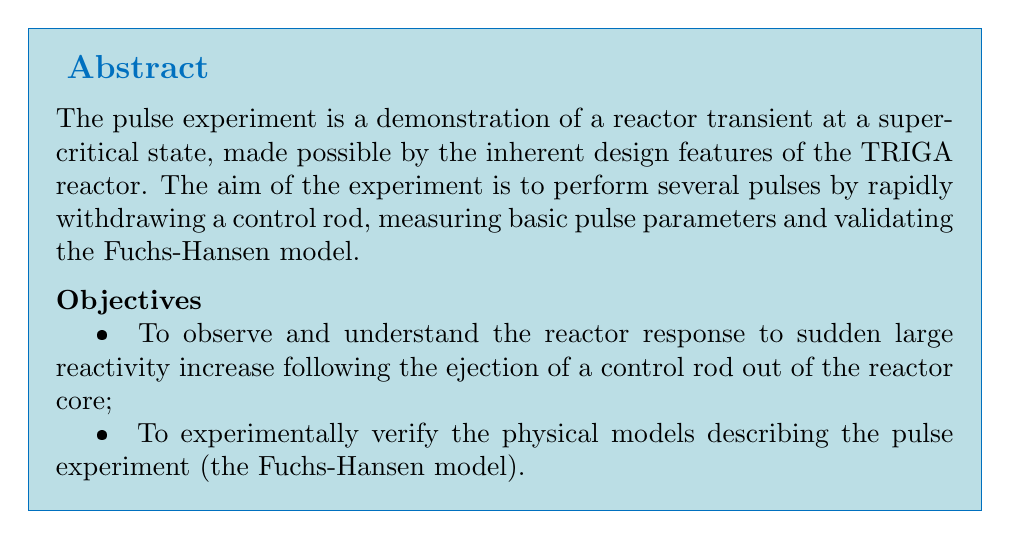
\begin{tikzpicture}
\coordinate (a) at (current page.north);%top of the page
\node [name=colourbar,
anchor=base,
fill=color-4,
fill opacity=0.5,
draw=color-3,
text = black,
text opacity=1,
align=justify,
text width=0.94\textwidth,
inner sep=10pt,
minimum height=2cm] at (a)
{
\begin{large}
\textbf{\color{color-3}Abstract}
\end{large}

\vspace{0.2cm}
The pulse experiment is a demonstration of a reactor transient at a supercritical state, made possible by the inherent design features of the TRIGA reactor. The aim of the experiment is to perform several pulses by rapidly withdrawing a control rod, measuring basic pulse parameters and validating the Fuchs-Hansen model.

\vspace{0.2cm}
\textbf{Objectives}

\hspace{0.5cm}•\hspace{0.2cm} To observe and understand the reactor response to sudden large reactivity increase following the ejection of a control rod out of the reactor core;

\hspace{0.5cm}•\hspace{0.2cm} To experimentally verify the physical models describing the pulse experiment (the Fuchs-Hansen model).

};

\end{tikzpicture}

\justifying

\color{color-3}

\tableofcontents

\vspace{4pt}
\noindent\rule[0.5ex]{\linewidth}{1pt}
\color{black}

\vspace{-1cm}



\section{Theory} % The \section*{} command stops section numbering

%\addcontentsline{toc}{section}{Theory} % Adds this section to the table of contents

Most of the TRIGA reactors are designed to enable pulse operation. One of the control rods, called the transient or pulse rod, can be very rapidly withdrawn out of the reactor core by a pneumatic ejection system. The reactor becomes promptly supercritical and the reactor power starts to increase exponentially with a very short time constant (period) of the order of a few milliseconds. The neutron population and the reactor power increases by several orders of magnitude and consequently the fuel temperature starts to rise. This increases the neutron absorption rate in fuel due to the Doppler broadening of resonances in $^{238}$U. Furthermore, since in TRIGAr reactors the fuel is homogeneously mixed with the moderator in the form of uranium-zirconium hydride (U-ZrH), the increase of fuel temperature also causes the fission rate to decrease due to the thermal neutron spectrum shift to higher energies. Both effects lead to significant reduction of reactivity and consequent reduction of reactor power back to low level. One can observe a short but intensive power excursion or pulse. Examples of time dependence of pulses following different reactivity insertions are shown in Fig. \ref{Fig:time}. \myfootnote{Authors of previous versions: Andrej Trkov, Matja\v z Ravnik, Ga\v sper \v Zerovnik}
\begin{figure}[ht!]
	\centering
	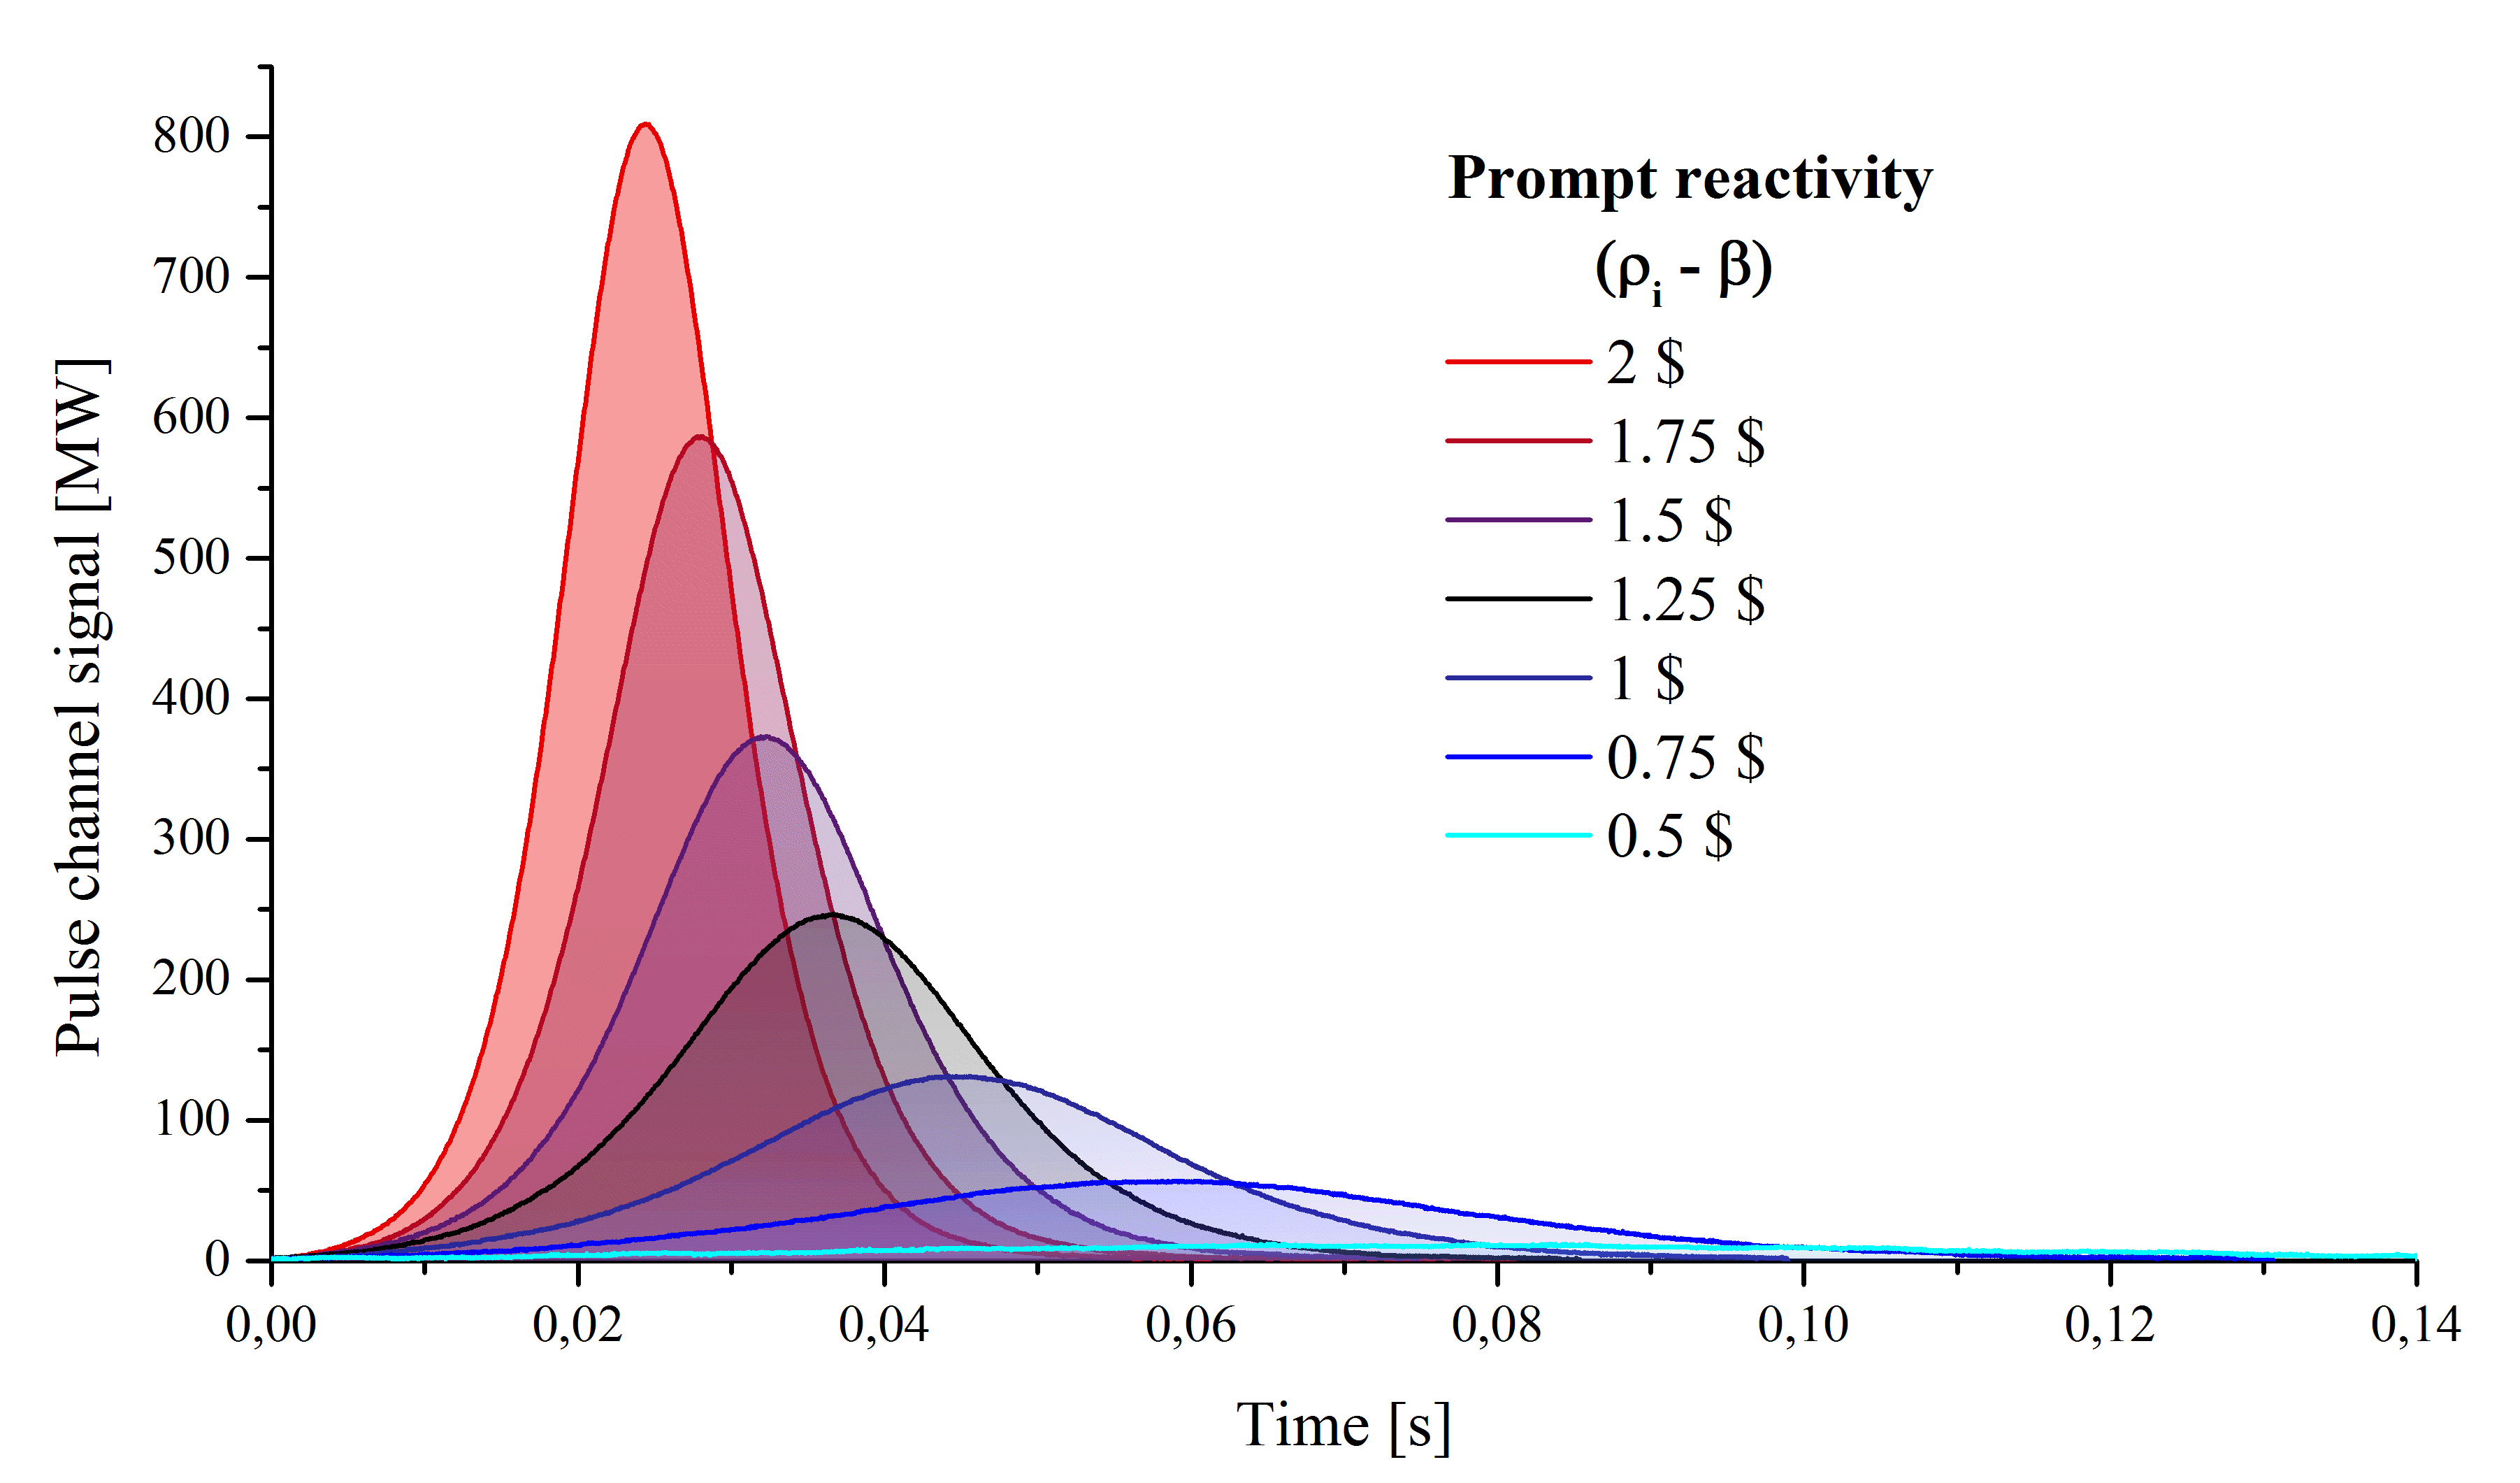
\includegraphics[width=0.8\textwidth]{slika2.png}
	\caption{Reactor power during a pulse experiment as a function of time from the beginning of the power rise. Pulses are indicated by prompt reactivity ranging from 2 \$ to 0.5 \$. The area under the pulse curve directly represents deposited energy used in the analysis [1].}
	\label{Fig:time}
\end{figure}

The total energy released during the pulse is relatively small (typically 1-10 $\mathrm{MWs}$) and does not damage the reactor in any way. The energy release and pulse height depends on the reactivity of the reactor after the rod withdrawal. The pulse rod is ejected to a pre-set position thereby defining the inserted reactivity. If the excess reactivity of the reactor is larger than the integral worth of the pulse rod, the pulse experiment can start at low-power critical reactor. If the excess reactivity is smaller, the pulse experiment starts with a subcritical reactor. The purpose of the exercise is to verify the relation between the pulse reactivity and basic pulse parameters, given by the theoretical model.

The time dependence of the pulse can be calculated using point kinetics equations by:
\begin{itemize}[noitemsep]
	\item neglecting the contribution of the delayed neutrons to the neutron population;
	\item assuming the reactivity decrease during the pulse is proportional to the energy release.
\end{itemize}

Both assumptions are physically justified since:
\begin{itemize}[noitemsep]
	\item the duration of the pulse ($\sim$ 10 $\mathrm{ms}$) is short compared to the decay times of the delayed neutron precursors ($\sim$ 10 $\mathrm{s}$);
	\item the duration of the pulse is so short that the heat removal from the fuel region is negligible.
\end{itemize}
This approximation is also called adiabatic, and the theoretical model is named after Fuchs and Hansen. The entire derivation is given in Ref. [2] (chapter \textit{9.6 LARGE POWER EXCURSION: The Fuchs-Hansen Model}). Here, only the important results are outlined for basic understanding and execution of the exercise:
\begin{itemize}[noitemsep]
	\item the pulse height is proportional to the square of the ‘\textit{prompt reactivity}’ $\rho’$ (Fig. \ref{Fig:f1}), 
	\item energy release is proportional to $\rho’$ (Fig. \ref{Fig:f2}), 
	\item the pulse width is inversely proportional to $\rho’$, 
	\item the reactor period immediately after the pulse rod withdrawal is inversely proportional to $\rho’$.
\end{itemize}
By definition, the prompt reactivity $\rho’$ equals the actual reactivity $\rho$ reduced by the effective delayed neutron fraction $\beta_{eff}$:
\begin{equation}
\rho’ = \rho - \beta_{eff}~~.
\end{equation}
\noindent The effective delayed neutron fraction depends on the properties of the fissile material in the fuel and slightly on the reactor geometry. For the TRIGA reactor at the Jožef Stefan Institute (JSI), $\beta_{eff}$ = 0.0074 = 740 $\mathrm{pcm}$. For the pulse experiment the reactivity is usually measured in units of $\beta$. This exercise is usually performed with prompt reactivity between 0 and 2$\beta$, although in principle higher reactivities are possible. The maximum reactivity is limited by the integral reactivity worth of the pulse rod and by the reactor operational limits and conditions.

The above relations, which are formally given by equations (9.82)-(9.89) in the Ref. [2], can be used to determine some of the physical properties of the reactor. For example, from the relation (9.89 Ref. [2]) between the total energy release and the prompt reactivity, the effective fuel temperature coefficient of reactivity $\gamma$ can be determined. Additionally, the prompt neutron lifetime $\Lambda$ can be determined from the equation for the pulse width at half-height or from equation (9.88 Ref. [2]) for the pulse height.

%------------------------------------------------

\section{Task}

Observe the reactor power and temperature response to sudden large reactivity increase.


%------------------------------------------------

\section{Equipment}

\begin{itemize}[noitemsep]
	\item Power indicator and other indicators at the reactor control panel
	\item Software for processing the time dependence of the power signal
\end{itemize}

%------------------------------------------------

\section{Instructions}

\subsection{General remarks}
Several pulses with different prompt reactivities will be performed. For each pulse, the following should be written down:
\begin{itemize}[noitemsep]
	\item pulse rod position after the launch (before it is always fully inserted),
	\item positions of all other control rods (which always remain unchanged during the pulse),
	\item reactor power before the pulse (it has to be negligible, $<$ 100 $\mathrm{W}$),
	\item fuel temperature before the pulse,
	\item reactor coolant temperature before and after the pulse,
	\item total energy release during the pulse,
	\item pulse peak height,
	\item maximum fuel temperature after the pulse.
\end{itemize}
All the required instrumentation is located at the reactor control panel. The prompt reactivity is determined from the reactivity, inserted by the pulse rod, which can be read from the pulse rod worth table (for the JSI TRIGA reactor see Appended additional material).

The time dependence of the pulses is obtained by processing the digitalized signals. The data is processed off-line (after the experiment). From the processed data, the pulse widths at half-height can be estimated.



\subsection{Results}
The most important relations to be studied with the results obtained:
\begin{itemize}[noitemsep]
	\item total energy release during the pulse as a function of prompt reactivity,
	\item maximum reactor power (at pulse peak) as a function of prompt reactivity,
	\item maximum fuel temperature after the pulse as a function of prompt reactivity,
	\item pulse widths at half-height as a function of prompt reactivity,
	\item effective fuel temperature coefficient of reactivity $\gamma$,
	\item prompt neutron lifetime $\Lambda$,
\end{itemize}
by using the Fuchs-Hansen model (Ref. [2]) with comments on uncertainties and C/M agreement.

%------------------------------------------------
\section{Questions}

\begin{itemize}[noitemsep]
	\item Why is the TRIGA reactor allowed to operate in the pulse mode?
	\item Under what circumstances does the Fuchs-Hansen model accurately describe the power excursion after the pulse rod ejection?
	\item Find some examples (e.g. from solid state physics, nuclear physics, biology, medicine, chemistry, or mechanical engineering), where useful measurements could be done by utilising the TRIGA pulse experiment! 
\end{itemize}

%----------------------------------------------------------------------------------------

\section{Sample measurements}

Sample measurements are presented in Fig. \ref{Fig:time}, Fig. \ref{Fig:f1}, Fig. \ref{Fig:f2} and Fig. \ref{Fig:f3}.



\begin{figure*}[ht!]
	\centering
	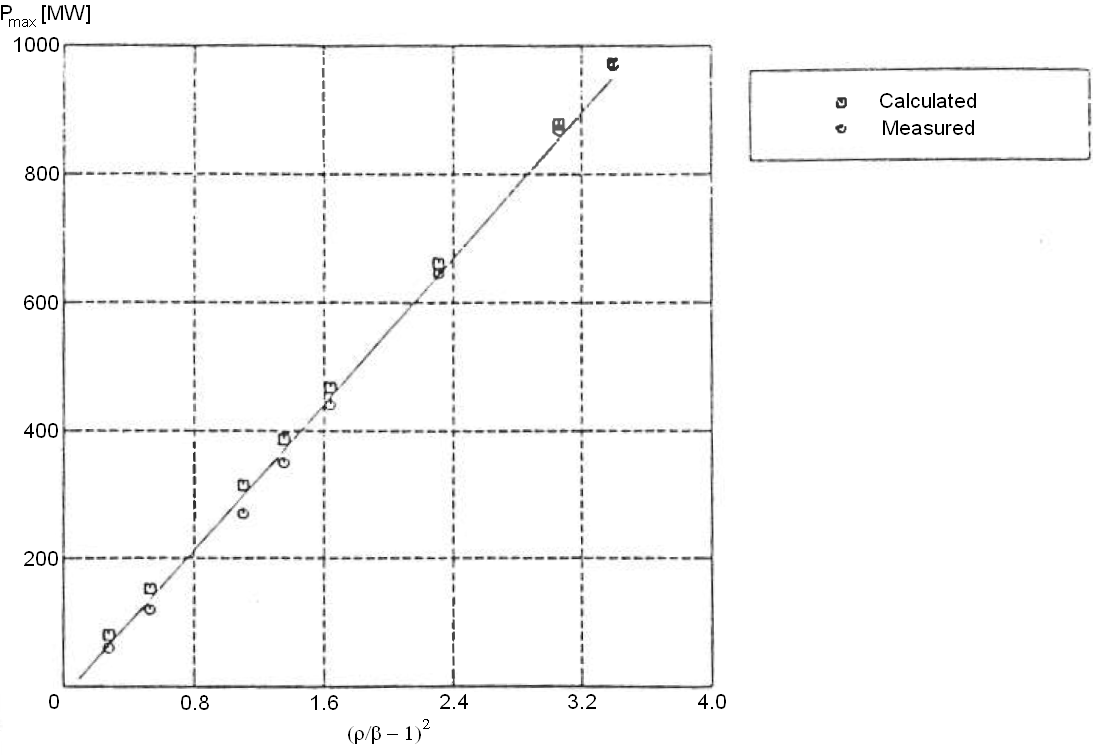
\includegraphics[width=0.8\textwidth]{fig1.png}
	\caption{Pulse peak height ($P_{max}$) as a function of the prompt reactivity squared (sample measurements from the JSI TRIGA reactor) [3].}
	\label{Fig:f1}
\end{figure*}

\begin{figure*}[ht!]
	\centering
	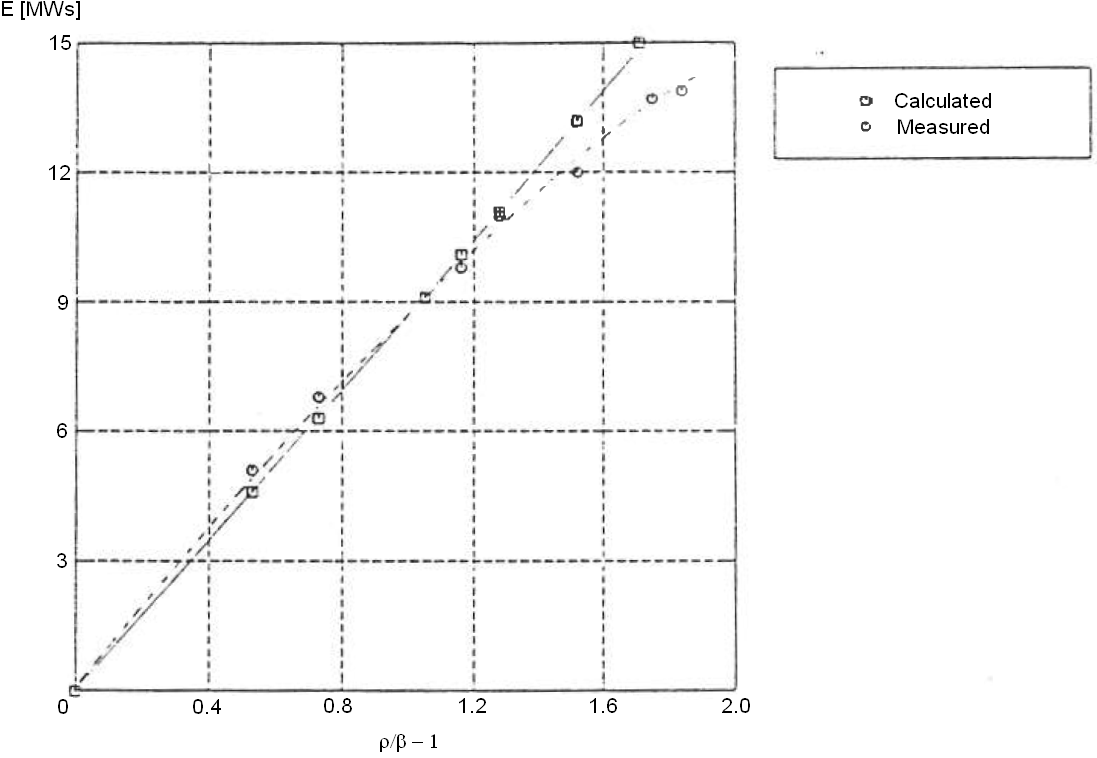
\includegraphics[width=0.8\textwidth]{fig2.png}
	\caption{Total energy release ($E$) during the pulse as a function of the prompt reactivity (sample measurements from the JSI TRIGA reactor) [3].}
	\label{Fig:f2}
\end{figure*}

\newpage

\begin{figure*}[ht!]
	\centering
	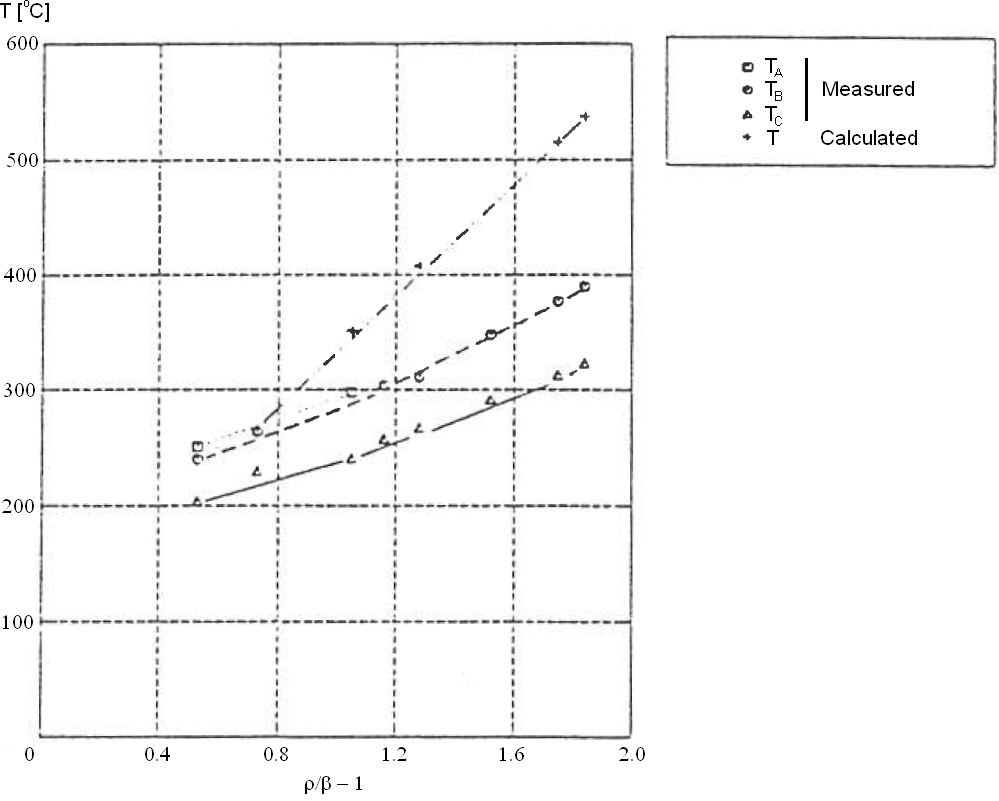
\includegraphics[width=0.8\textwidth]{fig3.png}
	\caption{Fuel temperature ($T$) after the pulse as a function of the prompt reactivity (sample measurements from the JSI TRIGA reactor) [3].}
	\label{Fig:f3}
\end{figure*}



\section{Appendix: Cherenkov Pulse Recorder}

\begin{wrapfigure}{r}{0.4\textwidth}
	\centering
	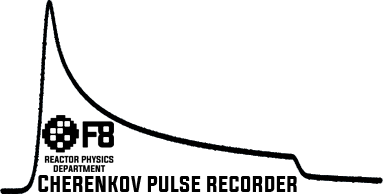
\includegraphics[width=0.4\textwidth]{logo.png}
	\caption{Cherenkov Pulse Recorder logo.}
	\label{fig:img1}
\end{wrapfigure}

In most water-cooled nuclear reactors, except zero-power reactors, Cherenkov radiation is present. It is due to energetic charged particles traveling faster than the speed of light in a dielectric medium. In open pool reactors, Cherenkov radiation can be observed as a blue glow around the reactor core. Since the intensity of the Cherenkov light produced in the reactor cooling water is in principle proportional to the neutron flux during a reactor pulse, an alternative method to measure the time dependence of the reactor power based on Cherenkov light intensity measurements is implemented at the JSI TRIGA research reactor.

\subsection{Equipment}

\begin{itemize}[noitemsep]
	\item Cherenkov pulse recorder
	\item Software for processing the time dependence of the Cherenkov light intensity signal
\end{itemize}

The Cherenkov Pulse Recorder is based on a closed tube in order to avoid interference from external light sources and radiation damage experienced by optical fibers. The system consists of an aluminium tube with an inner diameter of 36 mm positioned in the reactor core periphery, containing 0.65 l of water (filling the height of the reactor core in the tube). The water serves as the source of Cherenkov radiation in the measurement system. The Cherenkov light intensity in the channel is measured by silicon photo multiplier (SiPM) based detector linked with Redpitaya data acquisition system. With the use of neutral-density filters (ND filters), located in front of the SiPM dynamic range of the detector, is adjusted.

\subsection{Instructions}

\begin{itemize}[noitemsep]
	\item Connect with Redpitaya via browser (rp-f06ca3.local/)
	\item Start the SCPI server in the Development section
	\item Start Cherenkov Pulse Recorder software
	\item Initialize Cherenkov Pulse Recorder
	\item Adjust measuring parameters and start measurement
\end{itemize}

\noindent Raw measured signal is saved in CSV data file named: "pulse\_pulseNumber.csv". Measured pulse parameters are stored in CSV data file named: "recorded\_pulses\_Date.csv". During measurements signal should not reach $U_{max}=800$ mV. Apply appropriate ND filter if needed.

\begin{figure*}[ht!]
	\centering
	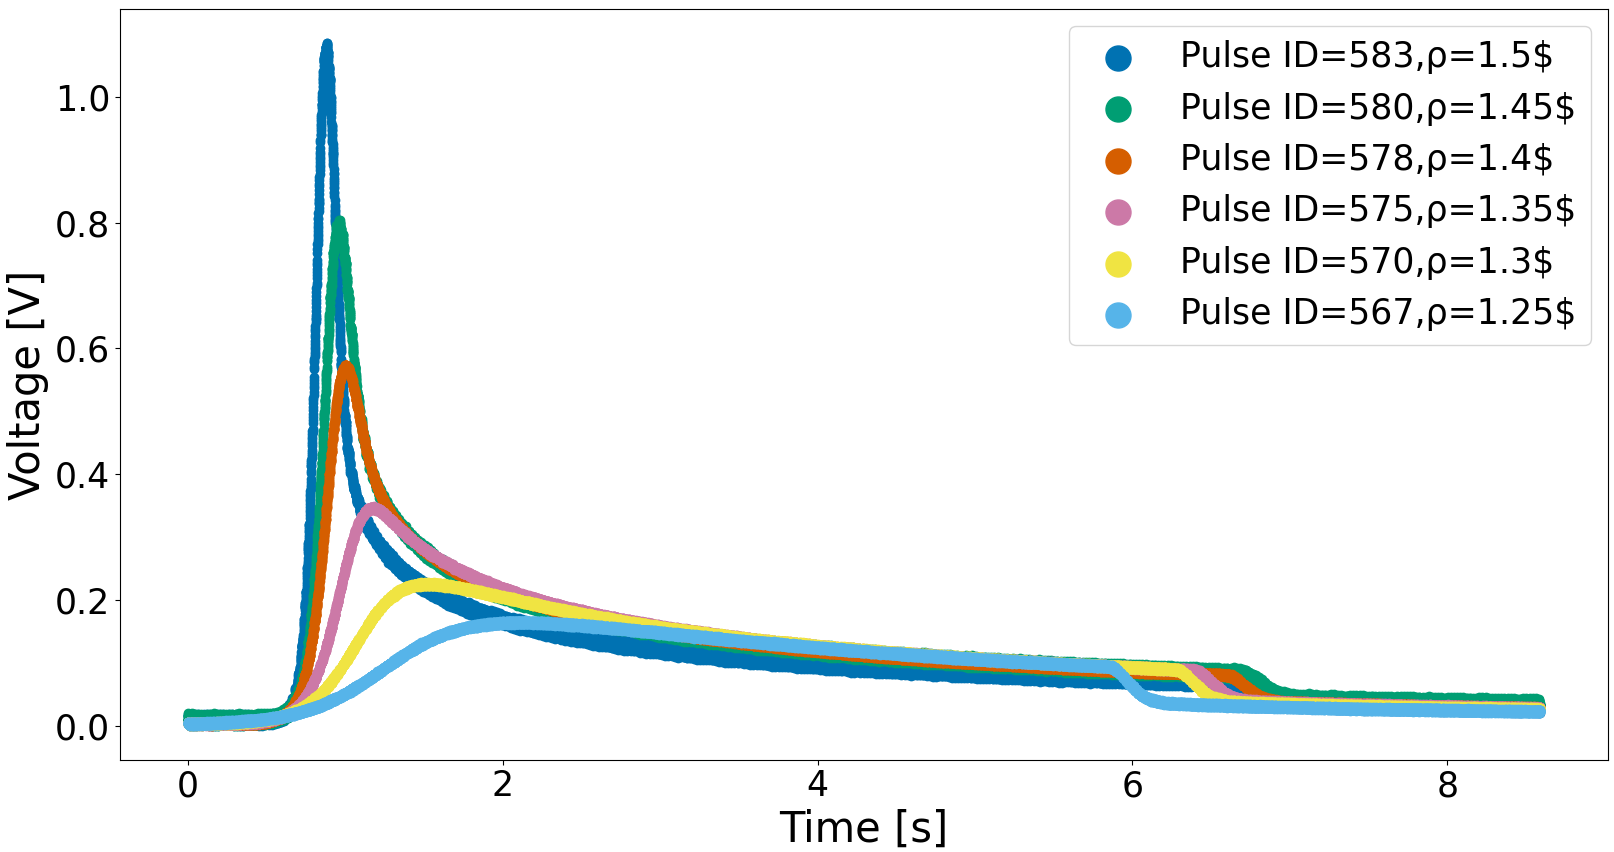
\includegraphics[width=0.99\textwidth]{fig4.png}
	\caption{Cherenkov Pulse Recorder signals during a pulse experiment as a function of time from the beginning of the power rise.}
	\label{Fig:f3}
\end{figure*}

%----------------------------------------------------------------------------------------
%	REFERENCE LIST
%----------------------------------------------------------------------------------------
\phantomsection
\begin{thebibliography}{99}
\bibitem{pung}
A. Punger\v ci\v c, I. Vavtar, L. Snoj, ''\textit{Analysis Of The JSI TRIGA Pulse Experiments}'', To be presented at: PHYSOR 2018: Reactor Physics paving the way towards more efficient systems, 2018.
\bibitem{Bell2001}
G. I. Bell, S. Glasstone, ''\textit{Nuclear Reactor Theory}'', Van Nostrand Reinhold Company, Litton Educational Publishing INC., New York, 1970.
\bibitem{ravnik}
I. Mele, M. Ravnik, A. Trkov, ''\textit{TRIGA Mark II Benchmark Experiment, Pert II: Pulse Operation}'', Nuclear Technology, 105, 1994.
\end{thebibliography}


\end{document}
